\section{Vorprojekt}
Der Fokus im Vorprojekt liegt auf der Erstellung der Benutzeroberfläche zur Erstellung eines Vierfachvordrucks. 
Die GUI wird über den Browser aufgerufen und ermöglicht in der Startseite die Auswahl der entsprechenden Rolle über 
ein Dropdown-Menü. In derselben Übersichtsseite sind die für die ausgewählte Rolle relevanten Informationen ersichtlich. 
Jede Rolle hat einen eigenen View. Beim Erstellen eines neuen Vordrucks soll das Design des Formulars im Vorprojekt 
weitestgehend fertig umgesetzt sein. Zu Demonstrationszwecken sollen einige voreingestellte Vordrucke zur Verfügung stehen. Neu erstellte Vordrucke bleiben zunächst nur temporär bestehen und gehen beim Verlassen der Seite verloren. Dadurch sollen Testnutzer in der Lage sein, einen ersten Überblick über den Prozess des Verfassens eines Vierfachvordrucks zu erhalten,
ohne sich Gedanken über die Integrität der Daten machen zu müssen. Der Workflow liegt hierbei zunächst nicht im Fokus; dieser wird erst im fertigen Projekt ersichtlich sein, da hierzu ein funktionsfähiges Backend benötigt wird.

    \begin{figure}[htpb]
        \centering
        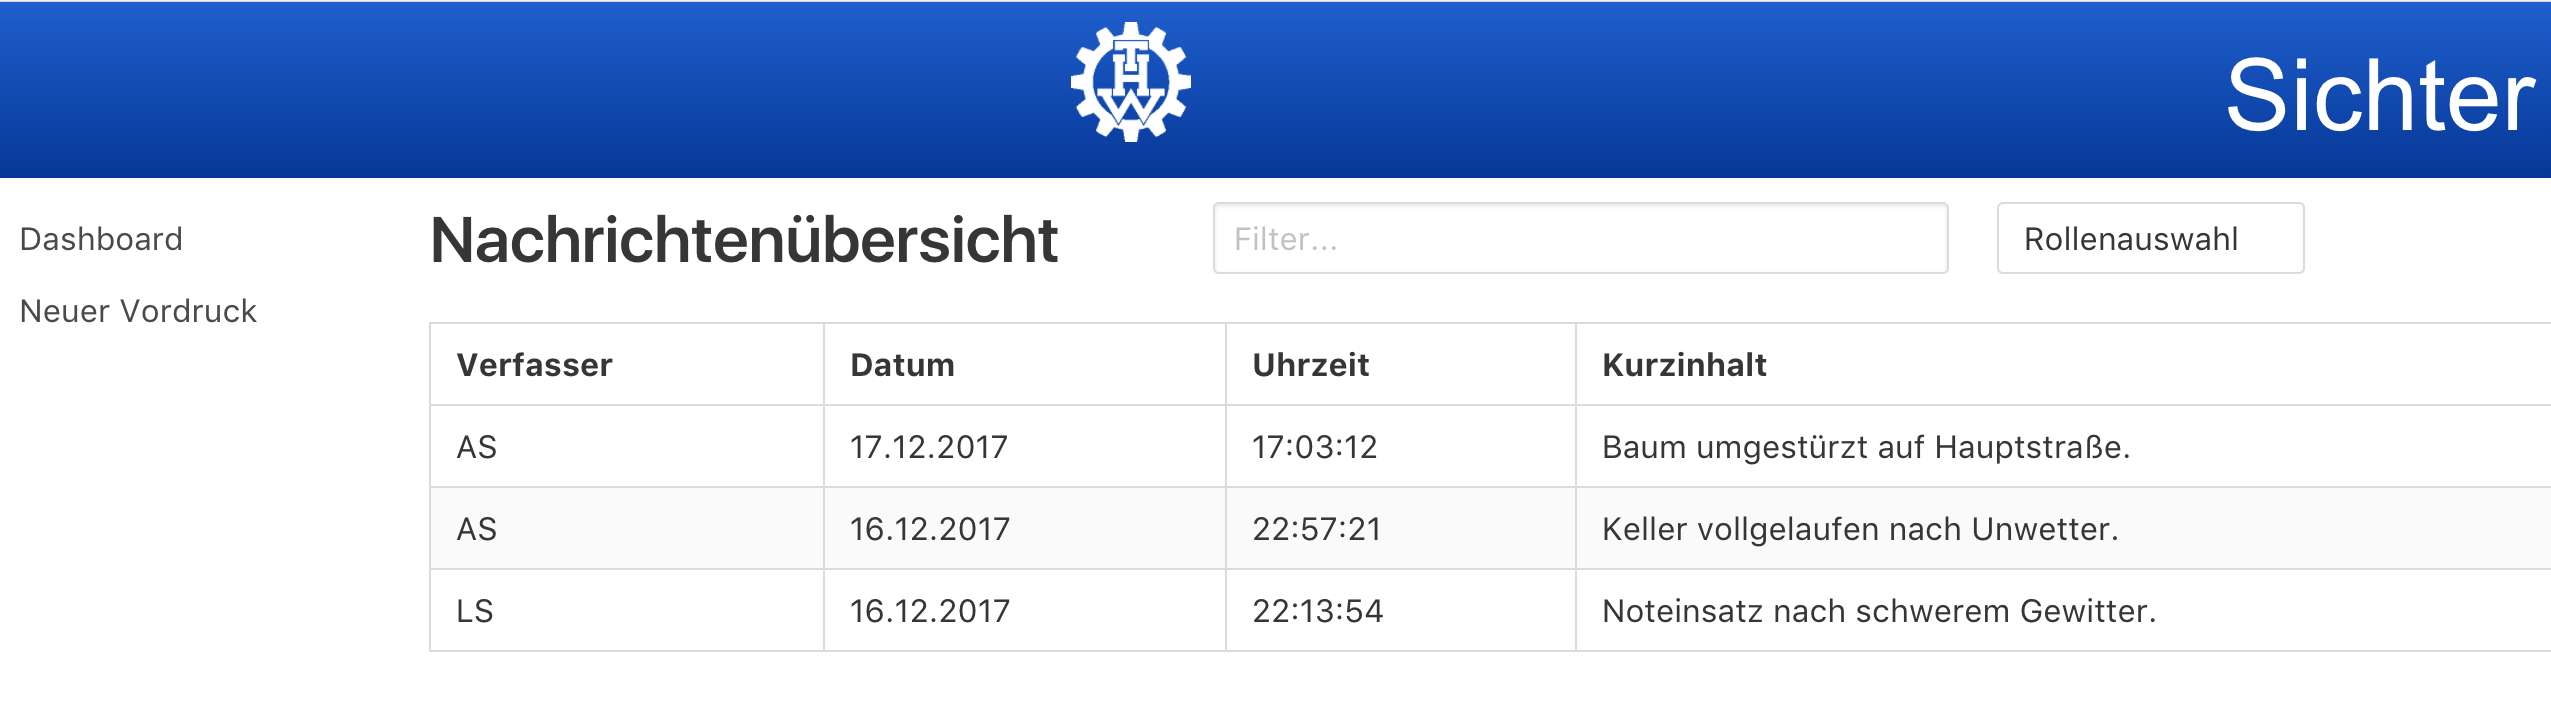
\includegraphics[width=0.95\linewidth]{vorprojekt_01.png}
        \caption{Startseite}
    \end{figure}


    \begin{figure}[htpb]
        \centering
        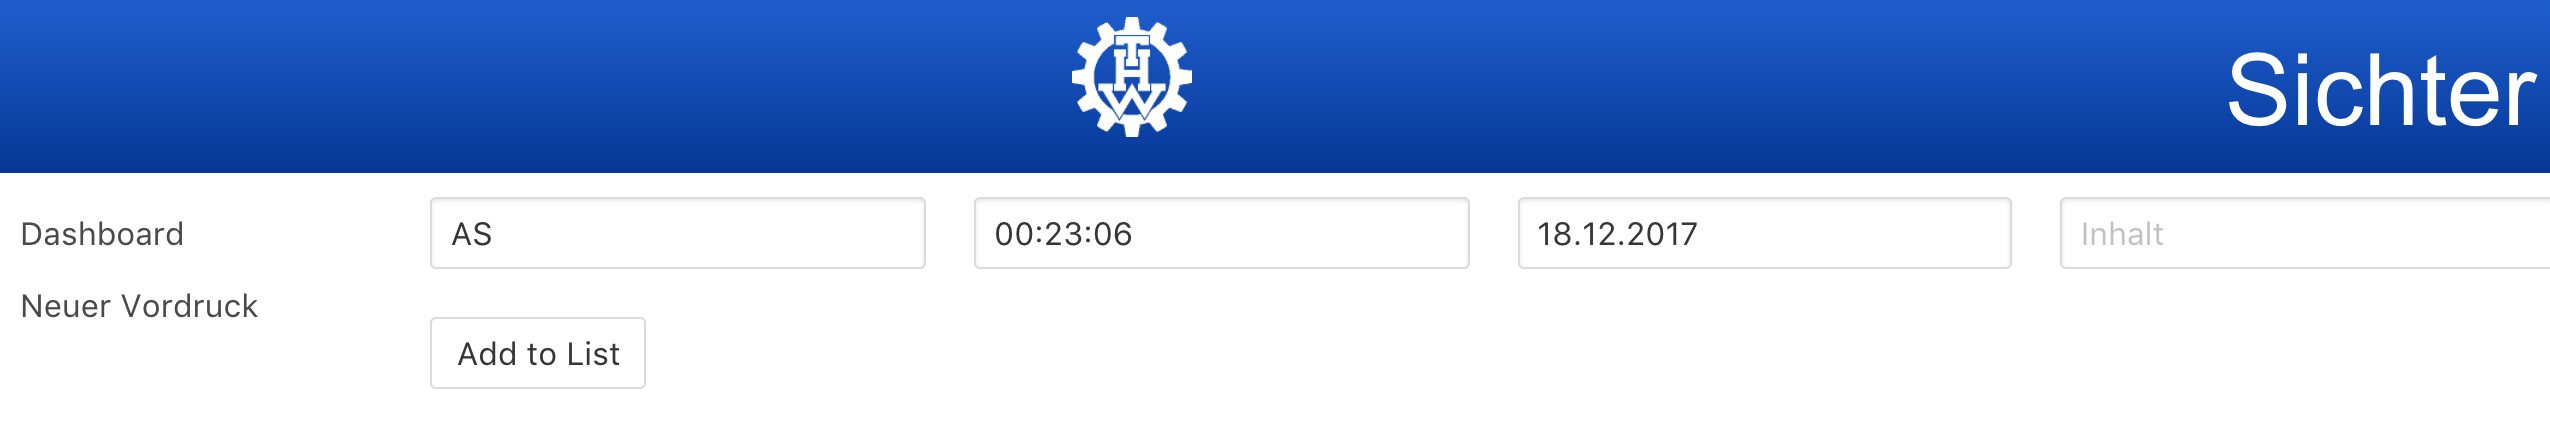
\includegraphics[width=0.95\linewidth]{vorprojekt_02.png}
        \caption{Erstellen eines neuen Vordrucks}
    \end{figure}
